\documentclass{deltares_memo}
\usepackage{CJKutf8}
\newcommand{\menuarrow}{$\rightarrow$}
\newcommand{\plotcfts}{PlotCFTS\xspace}
\newcommand{\qumesh}{QUmesh\xspace}
\newcommand{\netcdf}{netCDF\xspace}
\newcommand{\cfstandard}{Climate and Forecast 1.7 standard\xspace}

\newcommand\T{\rule{0pt}{2.6ex}}       % Top T
\newcommand\B{\rule[-1.2ex]{0pt}{0pt}} % Bottom T
\begin{document}
\memoTo{To whom it may concern}
\memoConfidentialUntil{}
\memoDate{\today}
\memoVersion{001}
\memoFrom{Jan Mooiman}
\memoTelephone{+31\,(0)88\,335\,8568}
\memoEmail{jan.mooiman@deltares nl}
\memoSubject{Manual to plot result files of \dflowfm in QGIS 3.12 (map- and history-files)}
\memoCopy{---}

\deltarestitle

%{{\footnotesize
%	{\textbf{Version control information}}
%	
%	\begin{tabular}{@{}p{12,5mm}@{}p{0mm}p{\textwidth-27mm-24pt}}
%		\textbf{Location} & \textbf{:} & \url{\svnkw{HeadURL}} \\
%		\textbf{Revision} & \textbf{:} & \svnrev 
%	\end{tabular}
%}}


\tableofcontents

%--------------------------------------------------------------------------------
\section{Release Notes}
\phantom{m}\vspace{-\baselineskip}
%
%--- begin light blue table ---
\begin{longtable}{p{16mm-12pt}|p{\textwidth-16mm-12pt}} 
%\caption{Light blue theme of table} \\% 
\rowcolor{dblue1} 
\textbf{Release} 
& \textbf{Description} 
\\ 
\topline 
\endfirsthead 
\endhead 
\endfoot 
\bottomline 
\endlastfoot 
0.00.00  &  - No information available.  \\
\end{longtable} 
%--- end light blue table ---
%
%--------------------------------------------------------------------------------
\section{Menu bar}
\phantom{m}\vspace{-\baselineskip}
\begin{figure}[H]
    \centering    
    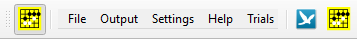
\includegraphics[width=0.40\textwidth]{pictures/menu_bar.png}
    \caption{The menu bar of the \qumesh plugin}
\end{figure}

%------------------------------------------------------------------------------
\subsection{File}
\phantom{m}\vspace{-\baselineskip}
\begin{figure}[H]
    \centering    
    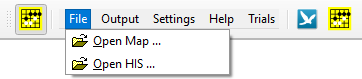
\includegraphics[width=0.40\textwidth]{pictures/menu_file.png}
    \caption{Menu \menuarrow File}
\end{figure}

%--------------------------------------------------------------------------------
\subsection{Output}
\phantom{m}\vspace{-\baselineskip}
\begin{figure}[H]
    \centering    
    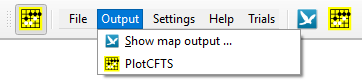
\includegraphics[width=0.40\textwidth]{pictures/menu_output.png}
    \caption{Menu \menuarrow Output}
\end{figure}

%------------------------------------------------------------------------------
\subsubsection{Show map output}
\phantom{m}\vspace{-\baselineskip}
\begin{figure}[H]
    \centering    
    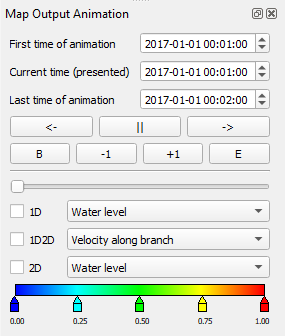
\includegraphics[width=0.5\textwidth]{pictures/map_output_animation_window.png}
    \caption{Map output animation window.}
\end{figure}

%------------------------------------------------------------------------------
\subsubsection{PlotCFTS}
After selecting this menu item the program \plotcfts will start.
\begin{figure}[H]
    \centering    
    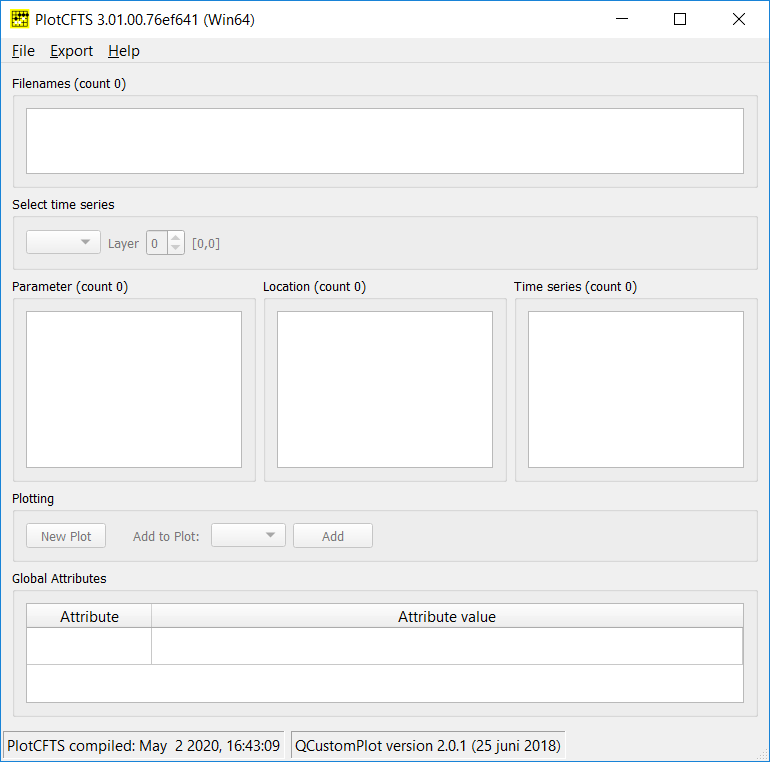
\includegraphics[width=0.9\textwidth]{pictures/main_plotcfts.png}
    \caption{Main window of the \plotcfts program.}
\end{figure}
%--------------------------------------------------------------------------------
\subsection{Settings}
\phantom{m}\vspace{-\baselineskip}
\begin{figure}[H]
    \centering    
    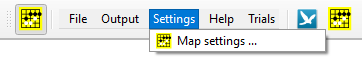
\includegraphics[width=0.40\textwidth]{pictures/menu_settings.png}
    \caption{Menu \menuarrow Settings}
\end{figure}
%--------------------------------------------------------------------------------
\subsection{Help}
\phantom{m}\vspace{-\baselineskip}
\begin{figure}[H]
    \centering    
    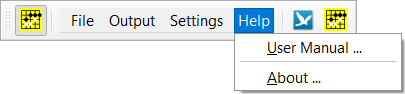
\includegraphics[width=0.4\textwidth]{pictures/menu_help.png}
    \caption{Menu \menuarrow Help}
\end{figure}

%--------------------------------------------------------------------------------
\subsubsection{User Manual}
Shows the user manual
\begin{figure}[H]
	\centering    
	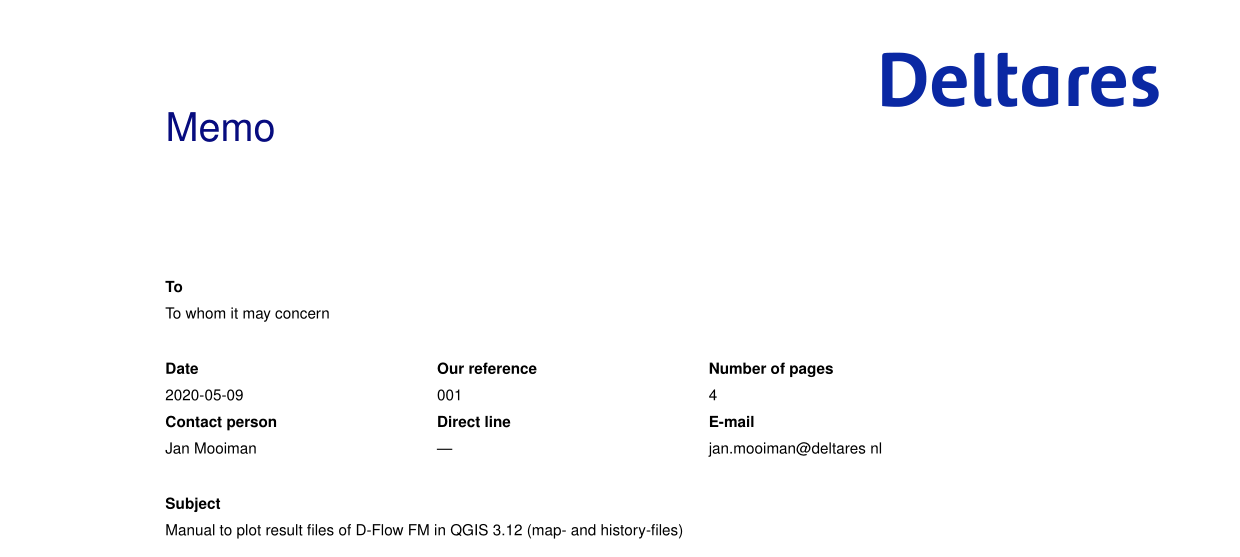
\includegraphics[width=0.9\textwidth]{pictures/menu_help_user_manual.png}
	\caption{\qumesh user manual}
\end{figure}

%--------------------------------------------------------------------------------
\subsubsection{About}
Shows the about box.
\begin{figure}[H]
    \centering    
    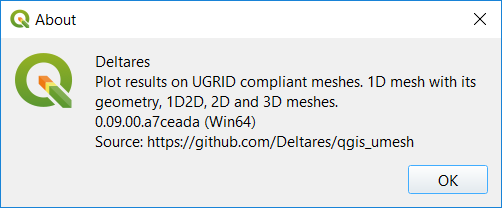
\includegraphics[width=0.4\textwidth]{pictures/menu_help_about.png}
    \caption{About box}
\end{figure}
%--------------------------------------------------------------------------------
\subsection{Trials}
\phantom{m}\vspace{-\baselineskip}
\begin{figure}[H]
    \centering    
    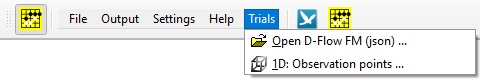
\includegraphics[width=0.40\textwidth]{pictures/menu_trials.png}
    \caption{Menu \menuarrow Trials}
\end{figure}
%------------------------------------------------------------------------------
\section{Source}
The source code is available on GitHUB:
\begin{Verbatim}
https://github.com/Deltares/qgis_umesh
\end{Verbatim}
%------------------------------------------------------------------------------

\end{document}
